\documentclass{beamer}

\title{EM Algorithm for Gaussian Mixture Model}
\date{April 2013}

\usetheme{CambridgeUK}

\begin{document}

\begin{frame}
\titlepage
\end{frame}

\section{Introduction}

\begin{frame}
\frametitle{Introduction of the Guassian Mixture Model}
\framesubtitle{Recap : The Guassian distribution}
The Guassian distribution:
\begin{equation}
\mathcal{N}(x | \mu, \Sigma) = \frac{1}{(2\pi)^{D/2}}\frac{1}{|\Sigma|^{1/2}}exp\{-\frac{1}{2}(x-\mu)^T\Sigma^{-1}(x-\mu)\}
\end{equation}
\begin{figure}
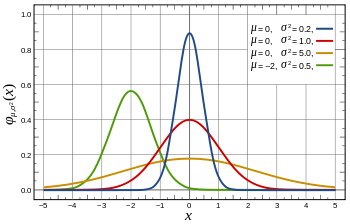
\includegraphics[width=200pt]{Guassian.png}
\end{figure}
\end{frame}

\begin{frame}
\frametitle{Introduction of the Guassian Mixture Model}
\framesubtitle{The Guassian Mixture distribution}
The Guassian Mixture distribution is a linear superposition of Guassians: 
\begin{equation}
p(x) = \Sigma^K_{k=1}\pi_k\mathcal{N}(x|\mu_k,\Sigma_k)
\end{equation}
Subject to:
\begin{equation}
\Sigma^K_{k=1}\pi_k = 1
\end{equation}
\begin{figure}
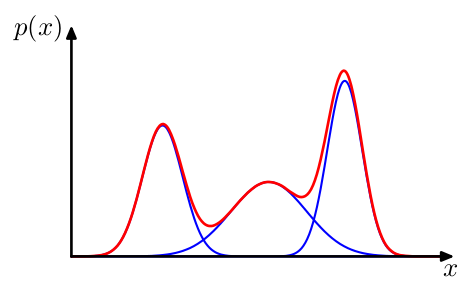
\includegraphics[width=170pt]{GMM-example2.png}\\
\end{figure}
\end{frame}

\begin{frame}
\frametitle{Introduction of the Guassian Mixture Model}
\framesubtitle{The Guassian Mixture distribution}
\begin{figure}
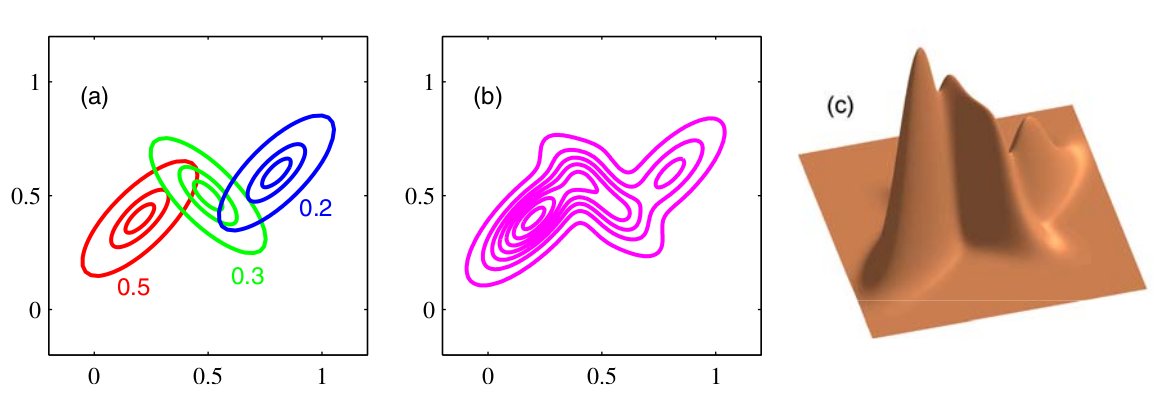
\includegraphics[width=330pt]{GMM-example.png}\\
A 2-dimension example of GMM
\end{figure}
\end{frame}

\begin{frame}
\frametitle{Introduction of the Guassian Mixture Model}
Now, for a Guassian Mixture Model, given the parameters:\\
$k$, the number of Guassian components\\
$\pi_1...\pi_k$, the mixture weights of the components\\
$\mu_1...\mu_k$, the mean of each component\\
$\Sigma_1...\Sigma_k$, the variance of each component\\
We can generate samples $s_1,s_2...s_n$ from the distribution.
\end{frame}

\begin{frame}
\frametitle{Why do we need Guassian Mixture}
\begin{figure}
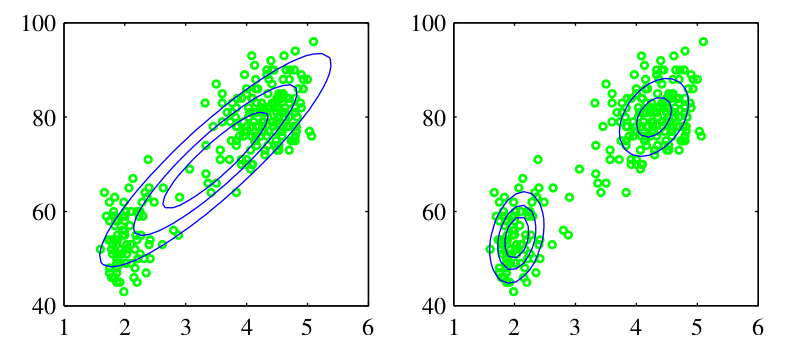
\includegraphics[width=300pt]{GMMbetterG.png}\\
In this example, we see that Guassian Mixture describes the data better a single Guassian.
\end{figure}
\end{frame}


\begin{frame}
\frametitle{Another representation of the Guassian Mixture}
Given a Guassian Mixture model, we introduce K-dimensional binary random variable z which only one element $z_k$ is euqal to 1 and the others are all 0.\\
\begin{equation}
z=(0,0,..,1,0,..0)
\end{equation}
So there are K possible states for z.And we let
\begin{equation}
p(z_k=1) = \pi_k
\end{equation}

\end{frame}


\begin{frame}
\frametitle{Even more structural elements}
\framesubtitle{Verse, Quote and Quotation}

\begin{verse}
This is a text in verse style.
\end{verse}

\begin{quote}
This is a quote.
\end{quote}

\begin{quotation}
While this is a quotation. Note how it has a larger indentation in the first line.
\end{quotation}

\end{frame}


\subsection{Maths}
\begin{frame}
\frametitle{Maths}
\framesubtitle{Including mathematical formulae into Beamer presentations is easy}

Beamer's biggest strength for scientific presentations is its ability to use the full power of \LaTeX's mathematical displays.

\begin{equation}
	\begin{aligned}
	D_{\text{KL}}(P_0, P_\infty) &= \sum_{\gamma\delta} P_0 ^{\gamma\delta} \log P_0 ^{\gamma\delta} - \sum_{\gamma\delta} P_0 ^{\gamma\delta} \log P_\infty ^{\gamma\delta}\\
					&= - H (P_0) - \langle \log P_\infty \rangle_0
	\label{eq:5}
	\end{aligned}
\end{equation}

\end{frame}

\begin{frame}\frametitle{Structuring Texts}
\framesubtitle{Lists}

\begin{columns}
\column{.5\textwidth}
\begin{enumerate}
	\item Of course Beamer can do enumerated lists
	\item It also knows how to do columns. This is helpful if you want to put figures next to text.
\end{enumerate}
\column{.5\textwidth}
\begin{itemize}
	\item bulleted lists are not numbered
	\item Beamer can do a lot more. For overlays, figures with captions, etc., have a look at \cite{Beamer}. But don't get carried away! Simple is nearly always better.
\end{itemize}

\end{columns}
\end{frame}

\begin{frame}{Installation Instructions}

These instructions assume you are using a packaged \LaTeX~distribution, like MikTex or TeXLive. If you have a custom installation, chances are you are proficient enough to interpret these instructions accordingly.

\begin{enumerate}
  \item install beamer. If you are using a \LaTeX~distribution, it's most probably already installed. Otherwise, see \cite{Beamer}
	\item find the beamer package directory. It's typically in [texroot]/tex/latex/beamer/. Change there.
	\item copy the file {\tt beamercolorthemecambridgeuk.sty} to ./themes/color/.
	\item copy the file {\tt beamerthemeCambridgeUK.sty} to ./themes/theme/.
	\item run {\tt sudo texhash}, or the equivalent on your system\footnote{Under MikTex on Windows, open Start $\to$ MikTex $\to$ Settings and run ``refresh FNDB''}
	
\end{enumerate}

\end{frame}

\section*{Bibliography}
\begin{frame}%[allowframebreaks] % add this if you have more papers to cite than fit on a slide.
\frametitle{Bibliography}

\begin{thebibliography}{Tantau, 2007}
\bibitem[aaPicutre]{Beamer}
Some pictures are from Wiki or PRML


\bibitem[Tantau, 2007]{Beamer}
Tantau, Till
\newblock {\em The Beamer class}
\newblock {\tt http://latex-beamer.sourceforge.net/}

\bibitem[Cambridge 2008]{UCGuide}
University of Cambridge
\newblock {\em Identity Guidelines -- first edition, May 2008}
\newblock {\tt http://www.admin.cam.ac.uk/offices/...\\ communications/services/identityguidelines/}

\end{thebibliography}
\end{frame}
\end{document}
